\documentclass{standalone}
\usepackage{tikz}
\usetikzlibrary{patterns, positioning}

\begin{document}
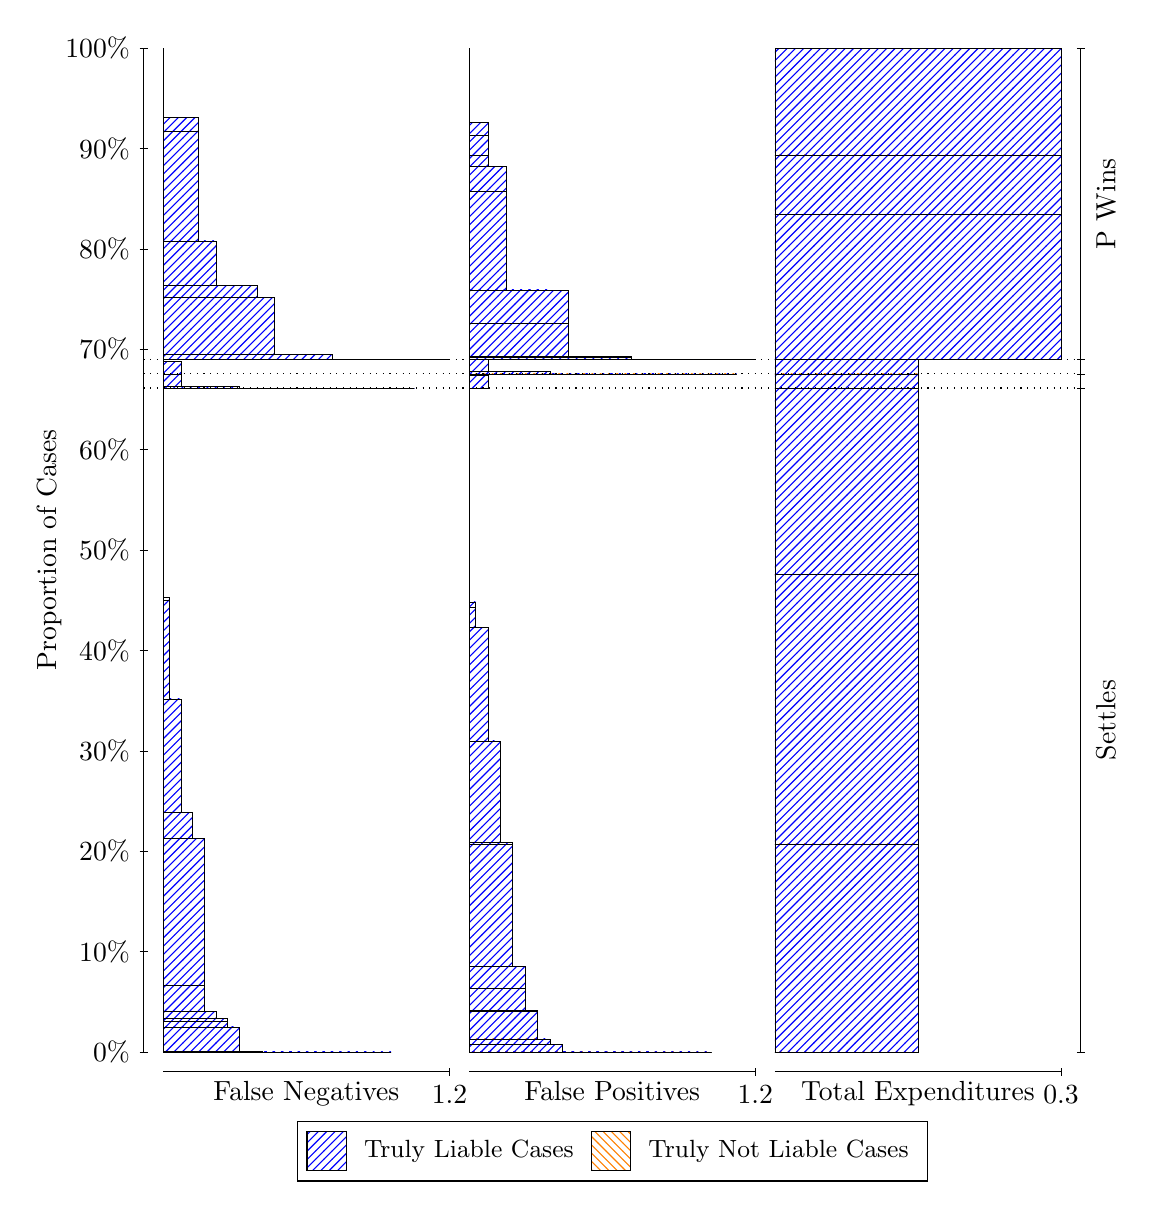
\begin{tikzpicture}
\draw[black, very thin] (1.5,1.75) -- (1.5,14.5);
\node[rotate=90, anchor=center] at (0.3, 8.125) {Proportion of Cases};
\draw[black, very thin] (1.45,1.75) -- (1.55,1.75);
\node[anchor=east] at (1.45, 1.75) {0\%};
\draw[black, very thin] (1.45,3.025) -- (1.55,3.025);
\node[anchor=east] at (1.45, 3.025) {10\%};
\draw[black, very thin] (1.45,4.3) -- (1.55,4.3);
\node[anchor=east] at (1.45, 4.3) {20\%};
\draw[black, very thin] (1.45,5.575) -- (1.55,5.575);
\node[anchor=east] at (1.45, 5.575) {30\%};
\draw[black, very thin] (1.45,6.85) -- (1.55,6.85);
\node[anchor=east] at (1.45, 6.85) {40\%};
\draw[black, very thin] (1.45,8.125) -- (1.55,8.125);
\node[anchor=east] at (1.45, 8.125) {50\%};
\draw[black, very thin] (1.45,9.4) -- (1.55,9.4);
\node[anchor=east] at (1.45, 9.4) {60\%};
\draw[black, very thin] (1.45,10.675) -- (1.55,10.675);
\node[anchor=east] at (1.45, 10.675) {70\%};
\draw[black, very thin] (1.45,11.95) -- (1.55,11.95);
\node[anchor=east] at (1.45, 11.95) {80\%};
\draw[black, very thin] (1.45,13.225) -- (1.55,13.225);
\node[anchor=east] at (1.45, 13.225) {90\%};
\draw[black, very thin] (1.45,14.5) -- (1.55,14.5);
\node[anchor=east] at (1.45, 14.5) {100\%};

\draw[black, very thin] (13.4,1.75) -- (13.4,14.5);
\draw[black, very thin] (13.35,1.75) -- (13.45,1.75);
\node[anchor=west] at (13.35, 1.75) {};
\draw[black, very thin] (13.35,10.182) -- (13.45,10.182);
\node[anchor=west] at (13.35, 10.182) {};
\draw[black, very thin] (13.35,10.362) -- (13.45,10.362);
\node[anchor=west] at (13.35, 10.362) {};
\draw[black, very thin] (13.35,10.543) -- (13.45,10.543);
\node[anchor=west] at (13.35, 10.543) {};
\draw[black, very thin] (13.35,14.5) -- (13.45,14.5);
\node[anchor=west] at (13.35, 14.5) {};

\draw[black, very thin, pattern color=blue, pattern=north east lines] (1.75,1.75) rectangle (4.6418,1.75);
\draw[black, very thin, pattern color=blue, pattern=north east lines] (1.75,1.75) rectangle (4.3452,1.75);
\draw[black, very thin, pattern color=blue, pattern=north east lines] (1.75,1.75) rectangle (4.0486,1.75);
\draw[black, very thin, pattern color=blue, pattern=north east lines] (1.75,1.75) rectangle (3.9003,1.75);
\draw[black, very thin, pattern color=blue, pattern=north east lines] (1.75,1.75) rectangle (3.752,1.75);
\draw[black, very thin, pattern color=blue, pattern=north east lines] (1.75,1.75) rectangle (3.6037,1.75);
\draw[black, very thin, pattern color=blue, pattern=north east lines] (1.75,1.75) rectangle (3.4554,1.7507);
\draw[black, very thin, pattern color=blue, pattern=north east lines] (1.75,1.7507) rectangle (3.3071,1.7508);
\draw[black, very thin, pattern color=blue, pattern=north east lines] (1.75,1.7508) rectangle (3.1588,1.7509);
\draw[black, very thin, pattern color=blue, pattern=north east lines] (1.75,1.7509) rectangle (3.0105,1.7509);
\draw[black, very thin, pattern color=blue, pattern=north east lines] (1.75,1.7509) rectangle (3.0105,1.7536);
\draw[black, very thin, pattern color=blue, pattern=north east lines] (1.75,1.7536) rectangle (2.8622,1.7593);
\draw[black, very thin, pattern color=blue, pattern=north east lines] (1.75,1.7593) rectangle (2.7139,2.0681);
\draw[black, very thin, pattern color=blue, pattern=north east lines] (1.75,2.0681) rectangle (2.5656,2.1338);
\draw[black, very thin, pattern color=blue, pattern=north east lines] (1.75,2.1338) rectangle (2.5656,2.1774);
\draw[black, very thin, pattern color=blue, pattern=north east lines] (1.75,2.1774) rectangle (2.4173,2.2679);
\draw[black, very thin, pattern color=blue, pattern=north east lines] (1.75,2.2679) rectangle (2.269,2.268);
\draw[black, very thin, pattern color=blue, pattern=north east lines] (1.75,2.268) rectangle (2.269,2.598);
\draw[black, very thin, pattern color=blue, pattern=north east lines] (1.75,2.598) rectangle (2.269,4.4655);
\draw[black, very thin, pattern color=blue, pattern=north east lines] (1.75,4.4655) rectangle (2.1207,4.7937);
\draw[black, very thin, pattern color=blue, pattern=north east lines] (1.75,4.7937) rectangle (1.9724,6.2328);
\draw[black, very thin, pattern color=blue, pattern=north east lines] (1.75,6.2328) rectangle (1.8241,7.4886);
\draw[black, very thin, pattern color=blue, pattern=north east lines] (1.75,7.4886) rectangle (1.8241,7.5196);
\draw[black, very thin, pattern color=orange, pattern=north west lines] (1.75,7.5196) rectangle (1.75,7.5196);
\draw[black, very thin, pattern color=blue, pattern=north east lines] (1.75,7.5196) rectangle (1.75,10.182);
\draw[black, very thin, pattern color=blue, pattern=north east lines] (1.75,10.182) rectangle (4.9384,10.182);
\draw[black, very thin, pattern color=blue, pattern=north east lines] (1.75,10.182) rectangle (4.1969,10.182);
\draw[black, very thin, pattern color=blue, pattern=north east lines] (1.75,10.182) rectangle (3.4554,10.182);
\draw[black, very thin, pattern color=blue, pattern=north east lines] (1.75,10.182) rectangle (2.7139,10.206);
\draw[black, very thin, pattern color=blue, pattern=north east lines] (1.75,10.206) rectangle (1.9724,10.362);
\draw[black, very thin, pattern color=orange, pattern=north west lines] (1.75,10.362) rectangle (1.75,10.362);
\draw[black, very thin, pattern color=blue, pattern=north east lines] (1.75,10.362) rectangle (1.9724,10.516);
\draw[black, very thin, pattern color=orange, pattern=north west lines] (1.75,10.516) rectangle (1.75,10.516);
\draw[black, very thin, pattern color=blue, pattern=north east lines] (1.75,10.516) rectangle (1.75,10.543);
\draw[black, very thin, pattern color=blue, pattern=north east lines] (1.75,10.543) rectangle (5.3833,10.543);
\draw[black, very thin, pattern color=blue, pattern=north east lines] (1.75,10.543) rectangle (4.6418,10.544);
\draw[black, very thin, pattern color=blue, pattern=north east lines] (1.75,10.544) rectangle (4.4194,10.544);
\draw[black, very thin, pattern color=blue, pattern=north east lines] (1.75,10.544) rectangle (3.9003,10.614);
\draw[black, very thin, pattern color=blue, pattern=north east lines] (1.75,10.614) rectangle (3.6779,10.614);
\draw[black, very thin, pattern color=blue, pattern=north east lines] (1.75,10.614) rectangle (3.1588,11.335);
\draw[black, very thin, pattern color=blue, pattern=north east lines] (1.75,11.335) rectangle (2.9364,11.484);
\draw[black, very thin, pattern color=blue, pattern=north east lines] (1.75,11.484) rectangle (2.4173,12.051);
\draw[black, very thin, pattern color=blue, pattern=north east lines] (1.75,12.051) rectangle (2.1949,13.445);
\draw[black, very thin, pattern color=blue, pattern=north east lines] (1.75,13.445) rectangle (2.1949,13.616);
\draw[black, very thin, pattern color=orange, pattern=north west lines] (1.75,13.616) rectangle (1.75,13.616);
\draw[black, very thin, pattern color=blue, pattern=north east lines] (1.75,13.616) rectangle (1.75,14.5);
\draw[black, very thin, pattern color=orange, pattern=north west lines] (5.6333,1.75) rectangle (8.7138,1.75);
\draw[black, very thin, pattern color=blue, pattern=north east lines] (5.6333,1.75) rectangle (8.7138,1.75);
\draw[black, very thin, pattern color=orange, pattern=north west lines] (5.6333,1.75) rectangle (8.3978,1.75);
\draw[black, very thin, pattern color=blue, pattern=north east lines] (5.6333,1.75) rectangle (8.3978,1.75);
\draw[black, very thin, pattern color=orange, pattern=north west lines] (5.6333,1.75) rectangle (8.0819,1.75);
\draw[black, very thin, pattern color=blue, pattern=north east lines] (5.6333,1.75) rectangle (8.0819,1.75);
\draw[black, very thin, pattern color=blue, pattern=north east lines] (5.6333,1.75) rectangle (7.9239,1.75);
\draw[black, very thin, pattern color=orange, pattern=north west lines] (5.6333,1.75) rectangle (7.7659,1.75);
\draw[black, very thin, pattern color=blue, pattern=north east lines] (5.6333,1.75) rectangle (7.7659,1.75);
\draw[black, very thin, pattern color=blue, pattern=north east lines] (5.6333,1.75) rectangle (7.608,1.75);
\draw[black, very thin, pattern color=orange, pattern=north west lines] (5.6333,1.75) rectangle (7.45,1.75);
\draw[black, very thin, pattern color=blue, pattern=north east lines] (5.6333,1.75) rectangle (7.45,1.7501);
\draw[black, very thin, pattern color=blue, pattern=north east lines] (5.6333,1.7501) rectangle (7.292,1.7501);
\draw[black, very thin, pattern color=orange, pattern=north west lines] (5.6333,1.7501) rectangle (7.1341,1.7501);
\draw[black, very thin, pattern color=blue, pattern=north east lines] (5.6333,1.7501) rectangle (7.1341,1.7509);
\draw[black, very thin, pattern color=orange, pattern=north west lines] (5.6333,1.7509) rectangle (7.1341,1.7509);
\draw[black, very thin, pattern color=blue, pattern=north east lines] (5.6333,1.7509) rectangle (7.1341,1.7513);
\draw[black, very thin, pattern color=blue, pattern=north east lines] (5.6333,1.7513) rectangle (6.9761,1.7514);
\draw[black, very thin, pattern color=orange, pattern=north west lines] (5.6333,1.7514) rectangle (6.8181,1.7514);
\draw[black, very thin, pattern color=blue, pattern=north east lines] (5.6333,1.7514) rectangle (6.8181,1.8513);
\draw[black, very thin, pattern color=blue, pattern=north east lines] (5.6333,1.8513) rectangle (6.6601,1.9165);
\draw[black, very thin, pattern color=orange, pattern=north west lines] (5.6333,1.9165) rectangle (6.5022,1.9165);
\draw[black, very thin, pattern color=blue, pattern=north east lines] (5.6333,1.9165) rectangle (6.5022,2.2728);
\draw[black, very thin, pattern color=blue, pattern=north east lines] (5.6333,2.2728) rectangle (6.5022,2.2758);
\draw[black, very thin, pattern color=blue, pattern=north east lines] (5.6333,2.2758) rectangle (6.3442,2.5538);
\draw[black, very thin, pattern color=blue, pattern=north east lines] (5.6333,2.5538) rectangle (6.3442,2.8354);
\draw[black, very thin, pattern color=orange, pattern=north west lines] (5.6333,2.8354) rectangle (6.1862,2.8354);
\draw[black, very thin, pattern color=blue, pattern=north east lines] (5.6333,2.8354) rectangle (6.1862,4.3816);
\draw[black, very thin, pattern color=blue, pattern=north east lines] (5.6333,4.3816) rectangle (6.1862,4.4126);
\draw[black, very thin, pattern color=blue, pattern=north east lines] (5.6333,4.4126) rectangle (6.0283,5.6994);
\draw[black, very thin, pattern color=blue, pattern=north east lines] (5.6333,5.6994) rectangle (5.8703,7.1384);
\draw[black, very thin, pattern color=blue, pattern=north east lines] (5.6333,7.1384) rectangle (5.7123,7.3913);
\draw[black, very thin, pattern color=blue, pattern=north east lines] (5.6333,7.3913) rectangle (5.7123,7.4667);
\draw[black, very thin, pattern color=blue, pattern=north east lines] (5.6333,7.4667) rectangle (5.6333,10.182);
\draw[black, very thin, pattern color=orange, pattern=north west lines] (5.6333,10.182) rectangle (5.8703,10.182);
\draw[black, very thin, pattern color=blue, pattern=north east lines] (5.6333,10.182) rectangle (5.8703,10.338);
\draw[black, very thin, pattern color=blue, pattern=north east lines] (5.6333,10.338) rectangle (5.6333,10.362);
\draw[black, very thin, pattern color=orange, pattern=north west lines] (5.6333,10.362) rectangle (9.0297,10.362);
\draw[black, very thin, pattern color=blue, pattern=north east lines] (5.6333,10.362) rectangle (9.0297,10.362);
\draw[black, very thin, pattern color=blue, pattern=north east lines] (5.6333,10.362) rectangle (8.2399,10.362);
\draw[black, very thin, pattern color=blue, pattern=north east lines] (5.6333,10.362) rectangle (7.45,10.362);
\draw[black, very thin, pattern color=blue, pattern=north east lines] (5.6333,10.362) rectangle (6.6601,10.389);
\draw[black, very thin, pattern color=blue, pattern=north east lines] (5.6333,10.389) rectangle (5.8703,10.543);
\draw[black, very thin, pattern color=orange, pattern=north west lines] (5.6333,10.543) rectangle (9.2667,10.543);
\draw[black, very thin, pattern color=blue, pattern=north east lines] (5.6333,10.543) rectangle (9.2667,10.543);
\draw[black, very thin, pattern color=orange, pattern=north west lines] (5.6333,10.543) rectangle (8.4768,10.543);
\draw[black, very thin, pattern color=blue, pattern=north east lines] (5.6333,10.543) rectangle (8.4768,10.543);
\draw[black, very thin, pattern color=blue, pattern=north east lines] (5.6333,10.543) rectangle (8.4768,10.543);
\draw[black, very thin, pattern color=orange, pattern=north west lines] (5.6333,10.543) rectangle (7.687,10.543);
\draw[black, very thin, pattern color=blue, pattern=north east lines] (5.6333,10.543) rectangle (7.687,10.569);
\draw[black, very thin, pattern color=blue, pattern=north east lines] (5.6333,10.569) rectangle (7.687,10.584);
\draw[black, very thin, pattern color=orange, pattern=north west lines] (5.6333,10.584) rectangle (7.45,10.584);
\draw[black, very thin, pattern color=blue, pattern=north east lines] (5.6333,10.584) rectangle (7.45,10.584);
\draw[black, very thin, pattern color=orange, pattern=north west lines] (5.6333,10.584) rectangle (6.8971,10.584);
\draw[black, very thin, pattern color=blue, pattern=north east lines] (5.6333,10.584) rectangle (6.8971,11.005);
\draw[black, very thin, pattern color=blue, pattern=north east lines] (5.6333,11.005) rectangle (6.8971,11.426);
\draw[black, very thin, pattern color=orange, pattern=north west lines] (5.6333,11.426) rectangle (6.6601,11.426);
\draw[black, very thin, pattern color=blue, pattern=north east lines] (5.6333,11.426) rectangle (6.6601,11.427);
\draw[black, very thin, pattern color=blue, pattern=north east lines] (5.6333,11.427) rectangle (6.6601,11.427);
\draw[black, very thin, pattern color=blue, pattern=north east lines] (5.6333,11.427) rectangle (6.1072,12.675);
\draw[black, very thin, pattern color=blue, pattern=north east lines] (5.6333,12.675) rectangle (6.1072,12.992);
\draw[black, very thin, pattern color=blue, pattern=north east lines] (5.6333,12.992) rectangle (5.8703,13.132);
\draw[black, very thin, pattern color=orange, pattern=north west lines] (5.6333,13.132) rectangle (5.8703,13.132);
\draw[black, very thin, pattern color=blue, pattern=north east lines] (5.6333,13.132) rectangle (5.8703,13.391);
\draw[black, very thin, pattern color=blue, pattern=north east lines] (5.6333,13.391) rectangle (5.8703,13.559);
\draw[black, very thin, pattern color=blue, pattern=north east lines] (5.6333,13.559) rectangle (5.6333,14.5);
\draw[black, very thin, pattern color=orange, pattern=north west lines] (9.5167,1.75) rectangle (11.333,1.75);
\draw[black, very thin, pattern color=blue, pattern=north east lines] (9.5167,1.75) rectangle (11.333,4.3925);
\draw[black, very thin, pattern color=orange, pattern=north west lines] (9.5167,4.3925) rectangle (11.333,4.3925);
\draw[black, very thin, pattern color=blue, pattern=north east lines] (9.5167,4.3925) rectangle (11.333,7.811);
\draw[black, very thin, pattern color=orange, pattern=north west lines] (9.5167,7.811) rectangle (11.333,7.811);
\draw[black, very thin, pattern color=blue, pattern=north east lines] (9.5167,7.811) rectangle (11.333,10.182);
\draw[black, very thin, pattern color=orange, pattern=north west lines] (9.5167,10.182) rectangle (11.333,10.182);
\draw[black, very thin, pattern color=blue, pattern=north east lines] (9.5167,10.182) rectangle (11.333,10.362);
\draw[black, very thin, pattern color=orange, pattern=north west lines] (9.5167,10.362) rectangle (11.333,10.362);
\draw[black, very thin, pattern color=blue, pattern=north east lines] (9.5167,10.362) rectangle (11.333,10.543);
\draw[black, very thin, pattern color=orange, pattern=north west lines] (9.5167,10.543) rectangle (13.15,10.543);
\draw[black, very thin, pattern color=blue, pattern=north east lines] (9.5167,10.543) rectangle (13.15,12.386);
\draw[black, very thin, pattern color=orange, pattern=north west lines] (9.5167,12.386) rectangle (13.15,12.386);
\draw[black, very thin, pattern color=blue, pattern=north east lines] (9.5167,12.386) rectangle (13.15,13.144);
\draw[black, very thin, pattern color=orange, pattern=north west lines] (9.5167,13.144) rectangle (13.15,13.144);
\draw[black, very thin, pattern color=blue, pattern=north east lines] (9.5167,13.144) rectangle (13.15,14.5);
\draw[black, dotted] (1.5,10.182) -- (13.4,10.182);
\draw[black, dotted] (1.5,10.362) -- (13.4,10.362);
\draw[black, dotted] (1.5,10.543) -- (13.4,10.543);
\draw[black, very thin] (1.75,1.5) -- (5.3833,1.5);
\node[anchor=north] at (3.5667, 1.5) {False Negatives};
\draw[black, very thin] (5.3833,1.45) -- (5.3833,1.55);
\node[anchor=north] at (5.3833, 1.45) {1.2};

\draw[black, very thin] (5.6333,1.5) -- (9.2667,1.5);
\node[anchor=north] at (7.45, 1.5) {False Positives};
\draw[black, very thin] (9.2667,1.45) -- (9.2667,1.55);
\node[anchor=north] at (9.2667, 1.45) {1.2};

\draw[black, very thin] (9.5167,1.5) -- (13.15,1.5);
\node[anchor=north] at (11.333, 1.5) {Total Expenditures};
\draw[black, very thin] (13.15,1.45) -- (13.15,1.55);
\node[anchor=north] at (13.15, 1.45) {0.3};

\node[black, centered, rotate=90] at (13.72, 5.9661) {Settles};


\node[black, centered, rotate=90] at (13.72, 12.521) {P Wins};

\draw (7.449999999999999,1.5) node[draw=none] (baseCoordinate) {};
\begin{scope}[align=center]
        \matrix[scale=0.5, draw=black, below=0.5cm of baseCoordinate, nodes={draw}, column sep=0.1cm]{
            \node[rectangle, draw, minimum width=0.5cm, minimum height=0.5cm, pattern=north east lines, pattern color=blue] {}; &
            \node[draw=none, font=\small] (B) {Truly Liable Cases}; &
            \node[rectangle, draw, minimum width=0.5cm, minimum height=0.5cm, pattern=north west lines, pattern color=orange] {}; &
            \node[draw=none, font=\small] (B) {Truly Not Liable Cases}; \\
            };
\end{scope}

\end{tikzpicture}
\end{document}